\section{Extended Kalman Filter}
\label{ekf_section}

In estimation theory, the extended Kalman filter (EKF) is the nonlinear version of the Kalman filter which linearizes about an estimate of the current mean and covariance. In the case of well defined transition models, the EKF has been considered to estimate the state. 
in this system we have a state and an observer these are given by equation.
$ X=AX +BU + W_d $  and $ Y=CX + W_n $
In this $ W_d $ is disturbance and $ W_n $ is the noise by sensor.
So Kalman filter is used judges between data be disturbance and noise.


If $W_d >> W_n$ that means disturbance amount is higher than noise hence state estimation can rely more on sensor data for mapping than on previous state. And sensor is more reliable.

if $W_n >> W_d$ that means noise amount is higher than disturbance hence state estimation can rely more on previous plot data for mapping than on sensor. And state is more reliable than sensor.

So according in paper we learned that non-linear system is defined as.

\begin{figure}[!htb]
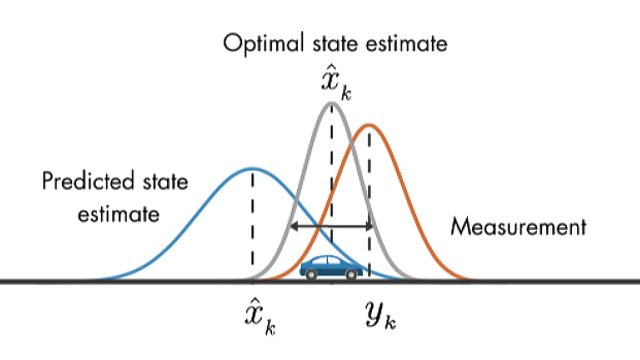
\includegraphics[width=\textwidth]{./figures/EKF.jpg}
\caption{Kalman filter state estimation~\cite{ByBo2015} }
\end{figure}

\begin{algorithm}
\caption{Kalman filter algorithm}\label{alg-gd}
\begin{algorithmic}[1]
\STATE Kalman Filter \({(\mu_{t-1},\Sigma_{t-1},u_t,z_t)}\)
\STATE \( {\mu_{t}}=A_t \mu_{t-1} + B_t u_t \)
\STATE \( \Sigma_{t}=A_t \Sigma_{t-1} A_t^T +R_t\)
\STATE \( K_t = \Sigma_{t} C_t(C_t^T \Sigma_{t}C_t^T+Q_t)^{-1}\)
\STATE \( \mu_{t}=\mu_{t}+K_t(z_t-C_t \mu_t) \)
\STATE \(\Sigma_{t}=(I-K_t C_t)\Sigma_{t}\)
\STATE return \( \mu_t ,  \Sigma_t \)
\end{algorithmic}
\end{algorithm}

So now lets take non-linear state equation as follows

\begin{equation}
\overrightarrow{z}_{k+1}= \overrightarrow{f}_k (\overrightarrow{z}_k) + v_k 
\end{equation}

\begin{equation} 
\begin{pmatrix}
  \overrightarrow{x}_{k+1} \\
  \overrightarrow{v}_{k+1} \\
  \overrightarrow{a}_{k+1} \\
  \overrightarrow{\lambda}_{k+1} \\
 \end{pmatrix}
 =
 \begin{pmatrix}
  I_3 & \frac{T}{\lambda}I_3  & \frac{T^2}{2 \lambda} I_3 & 0\\
  0 & I_3 & T I_3 & 0 \\
  0 & 0 & I_3 & 0 \\
  0 & 0 & 0 & 1\\
 \end{pmatrix} 
\begin{pmatrix}
\overrightarrow{x}_{k} \\
  \overrightarrow{v}_{k} \\
  \overrightarrow{a}_{k} \\
  \overrightarrow{\lambda}_{k} \\
 \end{pmatrix}
\end{equation}

where $x_k+1$ is the position without scale of the IMU/Camera and $v_{k+1}$ , $a_k+1$ are the velocity and acceleration of the IMU/Camera in metric unit [m]. $ν_k$ is the gaussian process noise. 
Main reason behind extended kalman filter working is when ever transition takes places between matices resultant output remains Gaussian and have defined mean and co-variance so in out treatment we can only do those transformation where we dont loose condition of system being Gaussian.
For example, Linear curve when transformed is Gaussian but if the function is non linear it is resultant does not result into Gaussian so whole point of using Kalman filter is killed.
So in Extended Kalman filter we linearize the system.
Every vector in $z_k$ is resolved in the world frame W. Note that we do not
include the orientation information in the model nor use it as a measurement in order. to keep the algorithm simple and fast. On each acceleration measurement we do the conversion from the inertial to the world frame by using a zero order hold  of the unfiltered attitude measurement returned by the visual SLAM framework. As we work in a middle size environment with enough loops we assume negligible drift win the SLAM map and assume thus highly accurate attitude estimation from the visual SLAM framework. The model in its linearized form yields,

\begin{figure}[!htb]
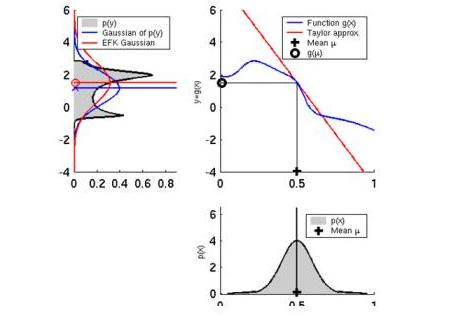
\includegraphics[width=\textwidth]{./figures/NonLinear.jpg}
\caption{Non-Linear system~\cite{ByBo2015}}
\end{figure}

\begin{equation}
F_k= 
 \begin{pmatrix}
  I_3 & \frac{T}{\lambda}I_3  & \frac{T^2}{2 \lambda} I_3& -\frac{T}{ \lambda^2} I_3 - \frac{T^2}{ 2 \lambda^2} I_3\\
  0 & I_3 & T I_3 & 0 \\
  0 & 0 & I_3 & 0 \\
  0 & 0 & 0 & 1\\
 \end{pmatrix} 
\end{equation}

For fusion implementation we consider the measurements in different observation
vectors. For a multi rate filter, as it is in our case, the literature suggests two solutions. One would be using a (higher order) hold to synchronize the different measurements. Another is to weight the uncertainty of the measurement according to its temporal occurrence. We claim no certainty at all if no
measurement is available (i.e. the measurement noise variance is infinite). Thus the update equations simplify to improve results. A more complex weighting function (i.e. exponential decay in time) could also be applied, however, at the cost of speed. The measurement updates for the vision and the IMU yields (‘V’ and ‘I’ denotes Vision and IMU)

The innovation done by authors in for the vision part is,
\begin{equation}
K_{V,k}=P_k^- H_{V,k}^T (H_{V,k} P_k H_{V,k}^T +R_v)^{-1}
\end{equation}
\begin{equation}
\overrightarrow{z}_{k}=\overrightarrow{z}_{k}+K_{V,k}(\overrightarrow{x}_{SLAM}-H_{V,k} \overrightarrow{z}_{k})
\end{equation}
\begin{equation}
P_k=(I-K_{V,k} H_{V,k}) P_k^-
\end{equation}

The innovation for by authors in the IMU part is,
\begin{equation}
K_{I,k}=P_k^- H_{I,k}^T (H_{I,k} P_k H_{I,k}^T +R_I)^{-1}
\end{equation}
\begin{equation}
\overrightarrow{z}_{k}=\overrightarrow{z}_{k}+K_{I,k}(\overrightarrow{x}_{IMU}-H_{I,k} \overrightarrow{z}_{k})
\end{equation}
\begin{equation}
P_k=(I-K_{I,k} H_{I,k}) P_k^-
\end{equation}

The two matrices $R_I$ , $R_V$ are the noise covariance matrices for the vision and IMU measurement inputs $x_{SLAM}$ , $a_{IMU}$ which are resolved in the world frame W.
The vector $x_{SLAM}$ is the position without scale obtained from the vision algorithm(SLAM). The IMU measurement $a_{IMU}$ needs special attention, because significant errors arise in the conversion from the raw IMU output.
\begin{equation}
\overrightarrow{a}_{w}=R_{wc}R_{ca} (\overrightarrow{a}_a - \overrightarrow{b})-\overrightarrow{g}_w
\end{equation}

